\documentclass[aspectratio=169,11pt]{beamer}
\usetheme{WestPoint}
\usepackage{booktabs}
\newcommand{\npts}{300}
\newcommand{\ntrain}{210}
\newcommand{\ntest}{90}
\newcommand{\acctwo}{54\%}
\newcommand{\accthree}{100\%}
\newcommand{\nsv}{5}


\title{Support Vector Machines}
\subtitle{Separating two rings with the kernel trick}
\author{Austin Semmel}
\institute{Department of Mathematical Sciences\\United States Military Academy}
\date{\today}

\begin{document}

\begin{frame}[plain]
  \titlepage
\end{frame}

% ---------------------------------------------------------------------------
\begin{frame}{The problem}
  \begin{columns}[c]
    \begin{column}{0.46\textwidth}\centering
      \includegraphics<1>[height=0.70\textheight]{figures/rings_2d.pdf}%
      \includegraphics<2>[height=0.70\textheight]{figures/rings_2d_line.pdf}%
    \end{column}
    \begin{column}{0.50\textwidth}
      \begin{itemize}
        \item \textbf{Data:} \npts{} points on two noisy rings, one inside the other
        \item \textbf{Split:} \ntrain{} points train the SVM; \ntest{} held-out points test it
        \item<2-> \textbf{Best straight line:} a linear SVM rates \acctwo{} of
          held-out points correctly, close to a coin flip
        \item<2-> Every line leaves part of the inner ring on the outer ring's side
      \end{itemize}
    \end{column}
  \end{columns}
\end{frame}

% ---------------------------------------------------------------------------
% Eleven overlays: the camera tilts from a top view into 3D, then the plane
% appears. In full-screen Acrobat the timings play it on their own.
\begin{frame}{Lift to 3D}
  \transduration<1-10>{0.25}
  \begin{columns}[c]
    \begin{column}{0.46\textwidth}\centering
      \includegraphics<1>[height=0.70\textheight]{figures/lift_01.pdf}%
\includegraphics<2>[height=0.70\textheight]{figures/lift_02.pdf}%
\includegraphics<3>[height=0.70\textheight]{figures/lift_03.pdf}%
\includegraphics<4>[height=0.70\textheight]{figures/lift_04.pdf}%
\includegraphics<5>[height=0.70\textheight]{figures/lift_05.pdf}%
\includegraphics<6>[height=0.70\textheight]{figures/lift_06.pdf}%
\includegraphics<7>[height=0.70\textheight]{figures/lift_07.pdf}%
\includegraphics<8>[height=0.70\textheight]{figures/lift_08.pdf}%
\includegraphics<9>[height=0.70\textheight]{figures/lift_09.pdf}%
\includegraphics<10>[height=0.70\textheight]{figures/lift_10.pdf}%
\includegraphics<11>[height=0.70\textheight]{figures/lift_11.pdf}%

    \end{column}
    \begin{column}{0.50\textwidth}
      \begin{itemize}
        \item Give every point a height:
          \[ \varphi(x_1, x_2) = \bigl(x_1,\ x_2,\ x_1^2 + x_2^2\bigr) \]
        \item Points far from the center rise higher, so the outer ring sits
          above the inner ring
        \item<11-> \textbf{A flat plane now separates them.} A linear SVM on the
          lifted points rates \accthree{} of held-out points correctly
      \end{itemize}
    \end{column}
  \end{columns}
\end{frame}

% ---------------------------------------------------------------------------
\begin{frame}{Back to 2D}
  \begin{columns}[c]
    \begin{column}{0.46\textwidth}\centering
      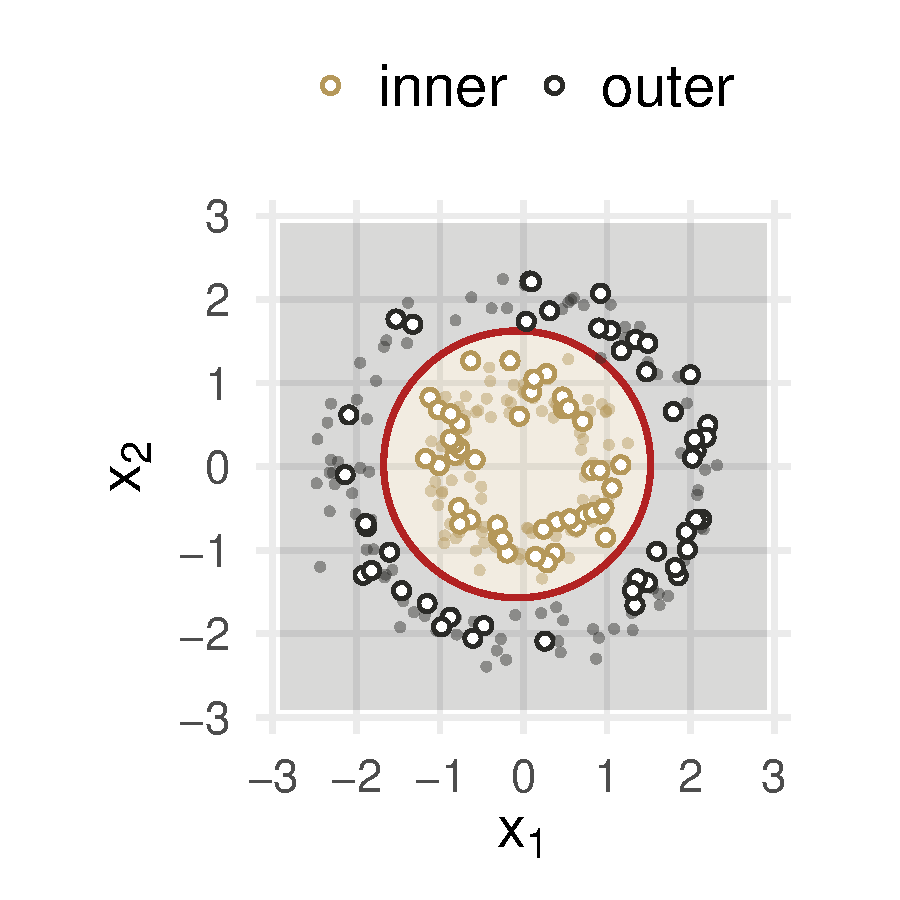
\includegraphics[height=0.70\textheight]{figures/rings_back.pdf}
    \end{column}
    \begin{column}{0.50\textwidth}
      \begin{itemize}
        \item The plane cuts the bowl in a circle, so the boundary in 2D is a circle
        \item Only \nsv{} support vectors set that boundary
      \end{itemize}
      \vspace{0.3em}
      \centering{\small\begin{tabular}{lc}
\toprule
\textbf{Linear SVM on} & \textbf{Held-out correct} \\
\midrule
$(x_1, x_2)$ & 54\% \\
$(x_1, x_2, x_1^2 + x_2^2)$ & 100\% \\
\bottomrule
\end{tabular}
}
      \vspace{0.2em}
      \begin{block}{The kernel trick}
        A kernel $K(\mathbf{x}, \mathbf{x}') = \varphi(\mathbf{x}) \cdot \varphi(\mathbf{x}')$
        gives the SVM this lift without computing $\varphi$.
      \end{block}
    \end{column}
  \end{columns}
\end{frame}

\end{document}
